\section{Results}
\label{sec:results}
\subsection{Data}
\label{sec:data}
We evaluate the proposed methods on data from the Human
Connectome Project (HCP) \cite{HCP}. The diffusion MR images have a resolution of $1.25$ mm
isotropic with $145 \times 174 \times 145$ voxels and have been acquired with 90 gradient directions each at $b\approx\{1000,2000,3000\}\,\mathrm{s}/\mathrm{mm}^2$.
%
We compare our results to reference tractographies which were published within the
scope of the TractSeg paper \cite{WASSERTHAL2018239}. This reference data has been
created by manually refining a segmented full brain fiber tractography. \added{Similar to TractSeg, we apply a variant of multi-shell multi-tissue deconvolution \cite{Jeurissen:2014,Ankele:CARS2017} that uses all available diffusion weighted images. It also yields per-voxel esimates of white matter volume fractions, which we threshold at $0.3$ to obtain the white matter masks used in our analyses.
}%For
%more details, we refer to the original literature.

All tests were performed on 12 randomly chosen subjects for which such reference tractographies
exist. For each tract, we created seed points by intersecting the reference
fiber bundle with a plane and initialize the tracking process with the direction
of the fiber bundle at the seed point. This should mimic a directional region of
interest as it might be defined by an expert on brain anatomy
\cite{Graumann2016}. We then apply the tracking process until we have as many
streamlines as the reference tractography. This should guarantee a fair comparison between the different models.

\added{Our comparison is between generic fiber tracking algorithms that can track from any given seed region. In contrast, bundle-specific approaches such as TractSeg are limited to reconstructing a predefined set of bundles, but have the benefit of tract-specific anatomical priors, which improve their accuracy.}

\subsection{Qualitative Comparison}
\begin{figure*}[t]
	\centering
	\begin{minipage}{0.19\linewidth}
\begin{subfigure}[b]{\linewidth}
		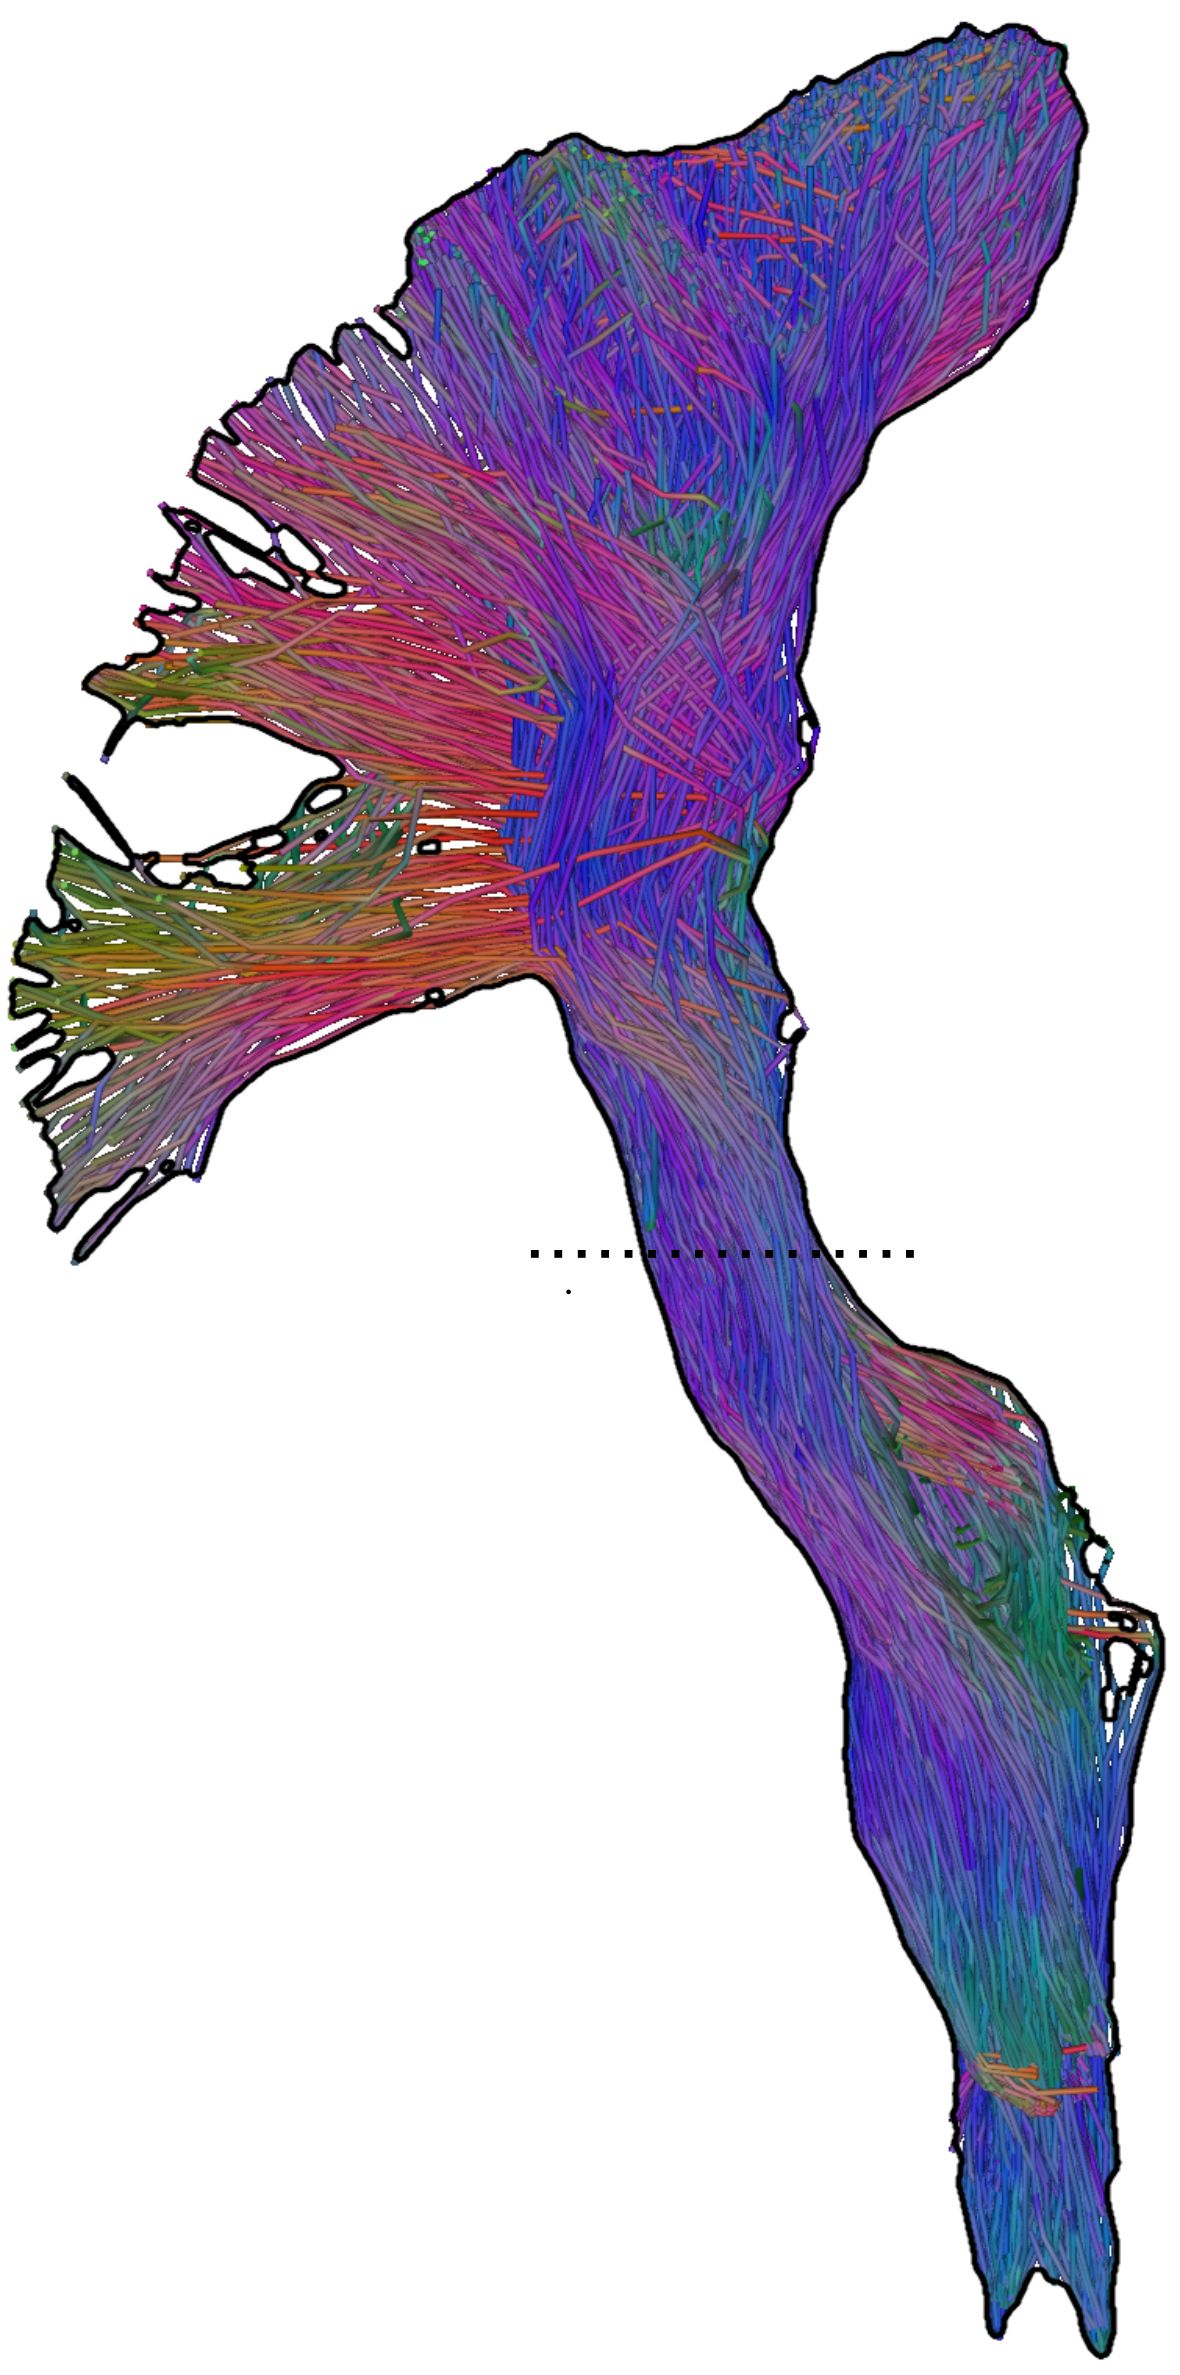
\includegraphics[width=\linewidth]{cst-ref-c}
		\caption{Reference with seed plane (dashed line)}
	\end{subfigure}
\end{minipage}
\hfil
	\begin{minipage}{0.19\linewidth}
		\begin{subfigure}[b]{\linewidth}
		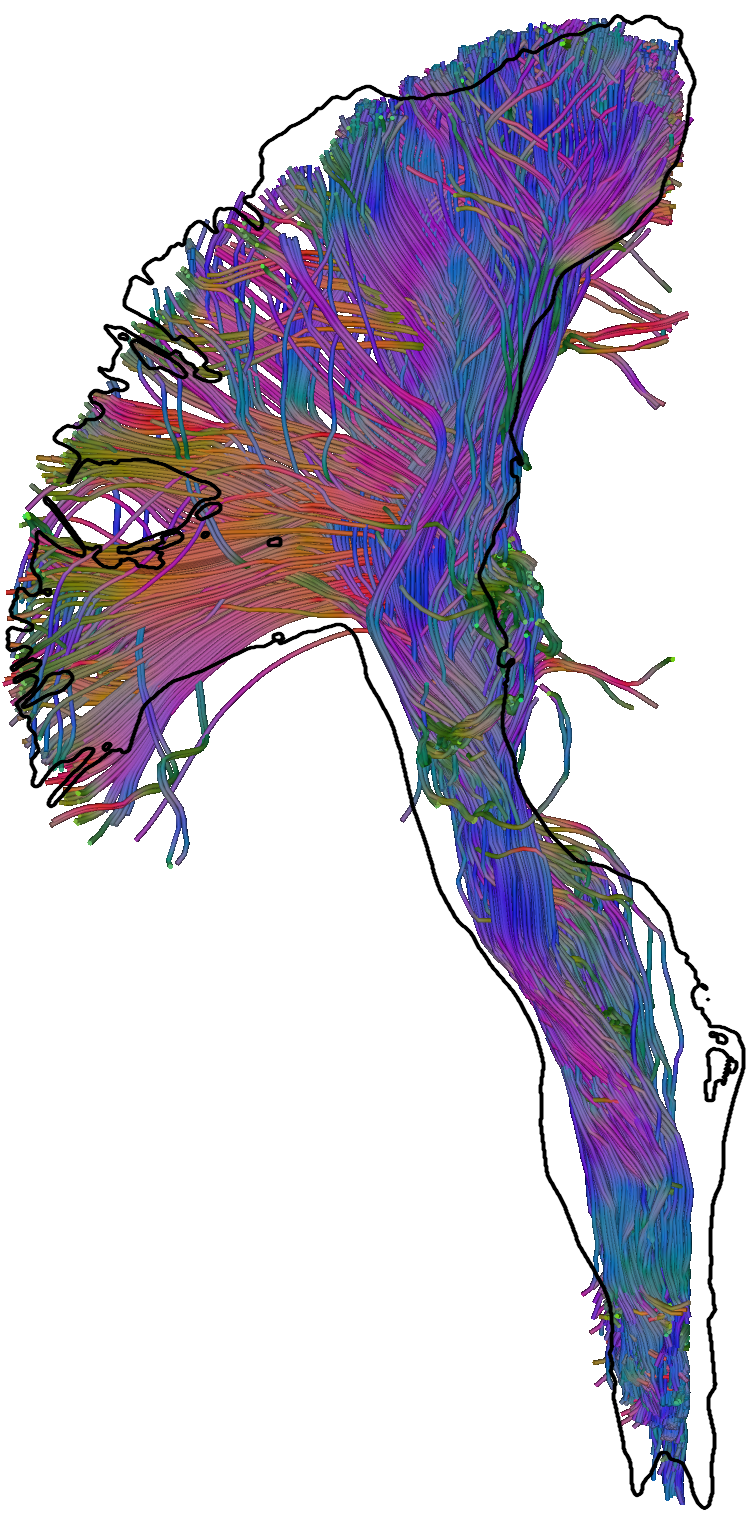
\includegraphics[width=\linewidth]{cst-rank-c}
		\caption{Low rank 3 model {\color{white} avdsdsds} }
	\end{subfigure}
	\begin{subfigure}[b]{\linewidth}
		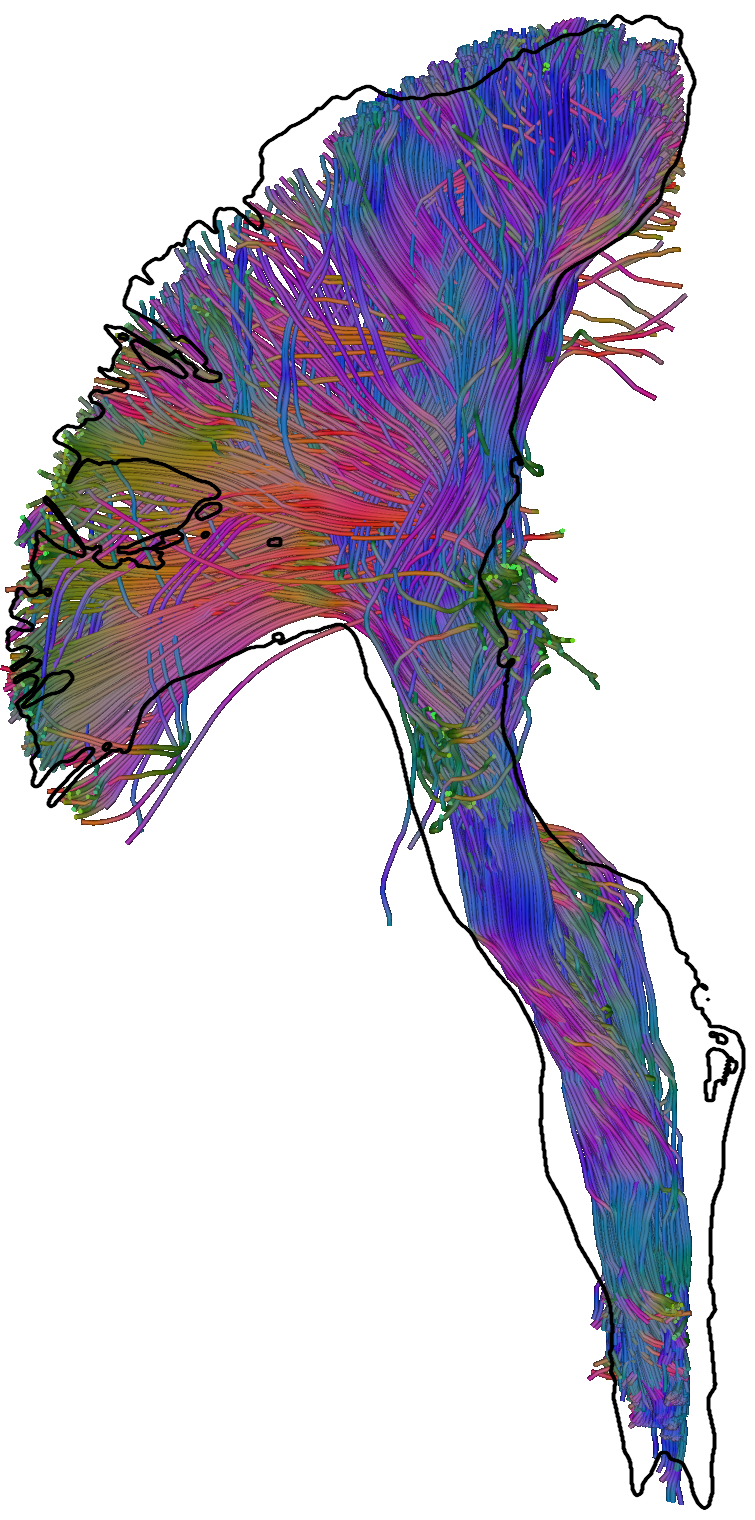
\includegraphics[width=\linewidth]{cst-rank-bootstrap-c}
		\caption{Consensus low rank 3 model}
\end{subfigure} 
	\end{minipage} \hfil
	\begin{minipage}{0.19\linewidth}
	\begin{subfigure}[b]{\linewidth}
		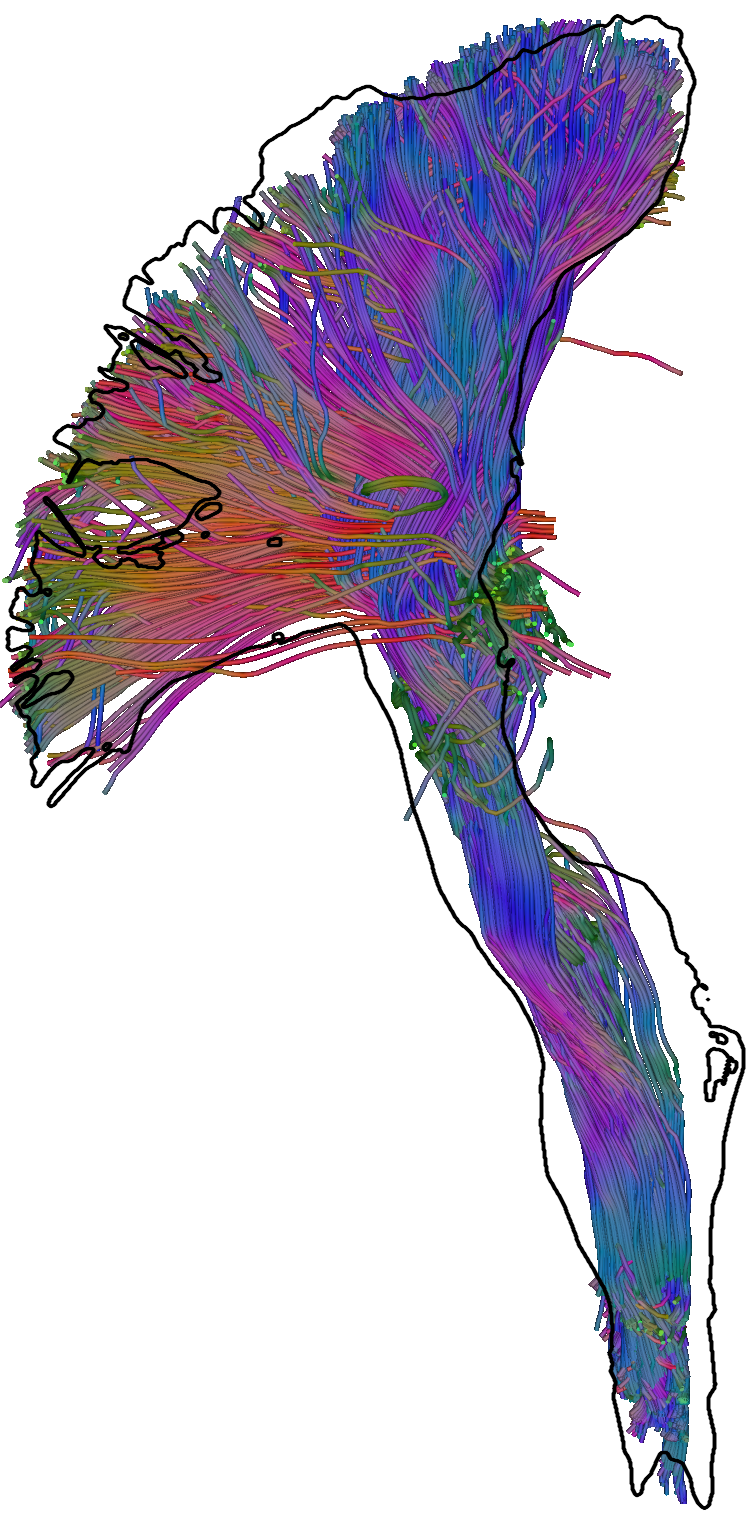
\includegraphics[width=\linewidth]{cst-avg-c}
		\caption{Average model {\color{white} aasfd vdsdsds}}
	\end{subfigure}
	\begin{subfigure}[b]{\linewidth}
		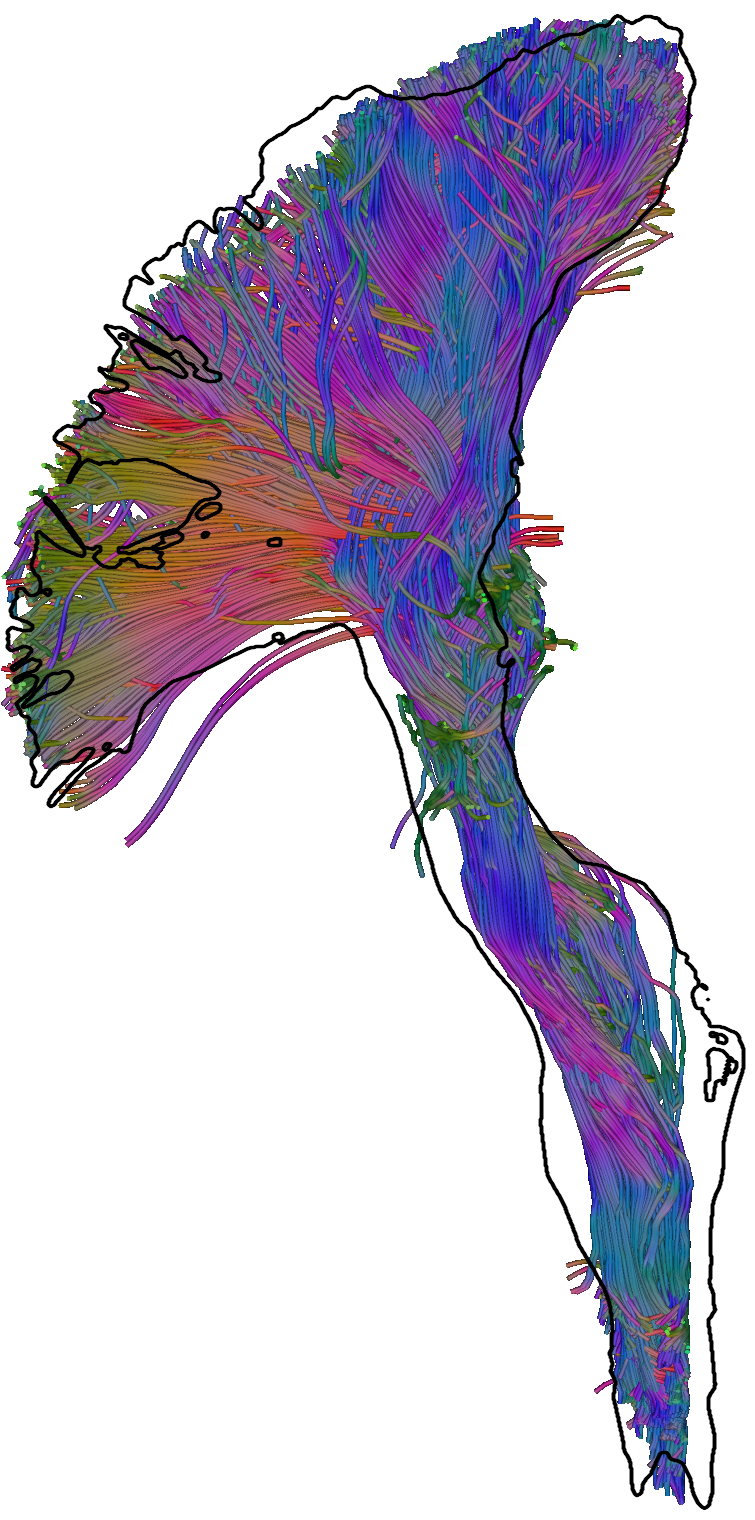
\includegraphics[width=\linewidth]{cst-avg-bootstrap-c}
		\caption{Consensus Average model{\color{white} aasfd vdsdsds}}
\end{subfigure} 
	\end{minipage} \hfil 
	\begin{minipage}{0.19\linewidth} 
	\begin{subfigure}[b]{\linewidth}
		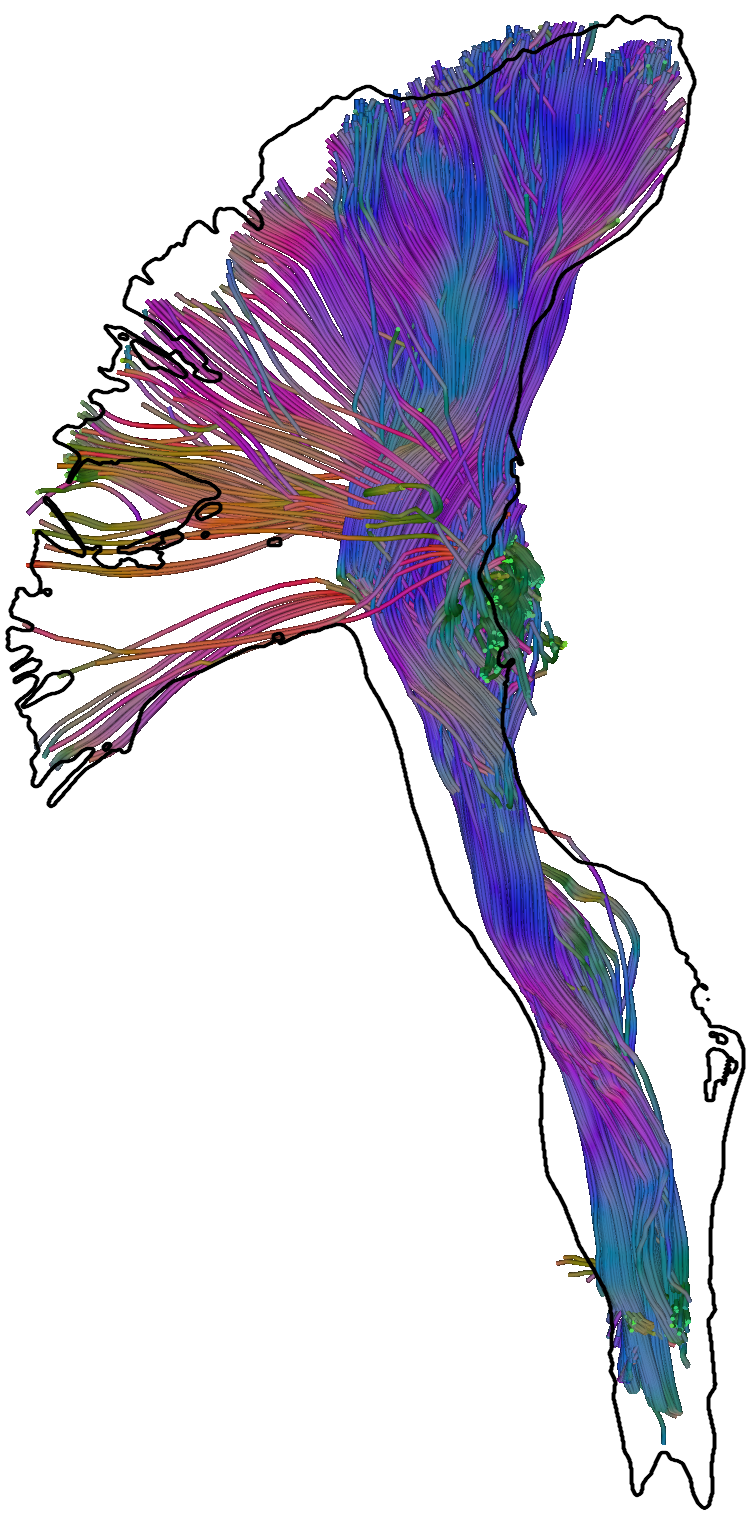
\includegraphics[width=\linewidth]{cst-sel-c}
		\caption{Selection model {\color{white} avdsdsds asdf asdf}}
	\end{subfigure}
	\begin{subfigure}[b]{\linewidth}
		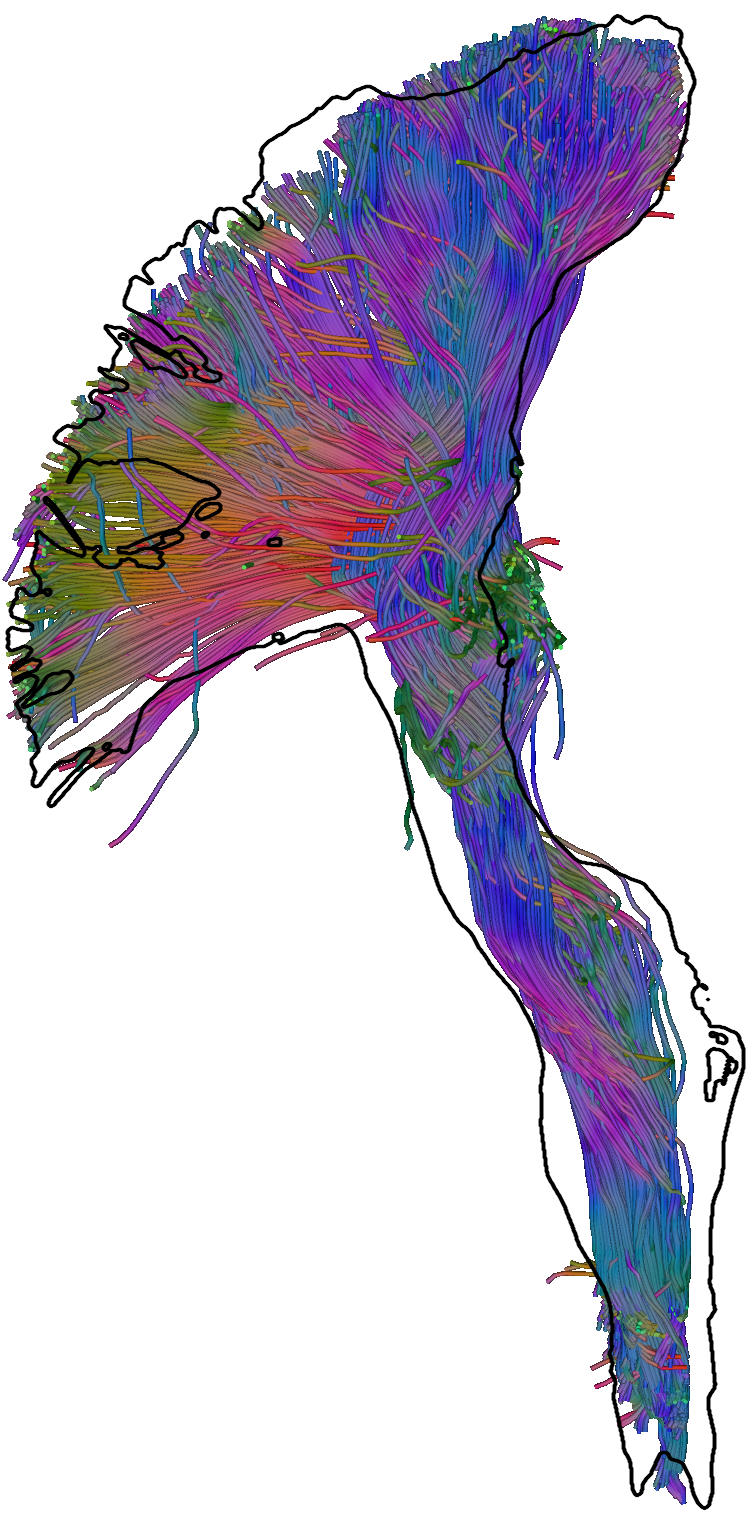
\includegraphics[width=\linewidth]{cst-sel-bootstrap-c}
		\caption{Consensus Selection Model}
\end{subfigure} 
	\end{minipage}
\caption{Reconstruction of the right corticospinal tract. For a more direct comparison
	between the reference and the tractographies, we overlaid the contour of the reference on each reconstruction with a black
	curve. The bootstrap consensus (bottom) leads to a much higher ability
to reconstruct the lateral spread compared to the base models (top). This is
especially true for the selection model (right).  }
	\label{fig:CST}
\end{figure*}

We compare results from model selection and model averaging, with and without the additional use of the bootstrap consensus. Our previous work \cite{Gruen:2021} included results from standard constrained spherical deconvolution as another baseline. However, this did not achieve competitive results and its computational expense made it difficult to combine it with bootstrapping. Therefore, we replaced it by a new baseline, which uses low-rank approximation with rank 3 throughout the brain.

As a first experiment, we track the right corticospinal tract (CST). We attempt to reconstruct the reference result, shown in Fig.~\ref{fig:CST}a, from a seed
region which is indicated with a dashed black line. To provide further guidance for visual comparison, the outline of the reference is overlaid on the remaining reconstructions as a black contour.

The main risk of a model selection strategy~(f) is premature tract termination due to a local underestimation of the true fiber number. It is obvious that this prevented full recovery of the lateral spread of the CST. Model averaging~(d) and bootstrap consensus~(g) both lead to more complete reconstructions. The bootstrap consensus leads to an ever denser sampling of the spreading region even when combining it with model averaging or the rank-3 model. An important advantage of model averaging compared to the rank-3 model is the reduction of false positives. This is less obvious in the image, because most of them have been filtered out successfully by the mechanisms in Section~\ref{sec:postprocessing}. However, it is clear from running times, which will be reported in Section~\ref{sec:computational-effort}.

\begin{figure*}
	\centering
	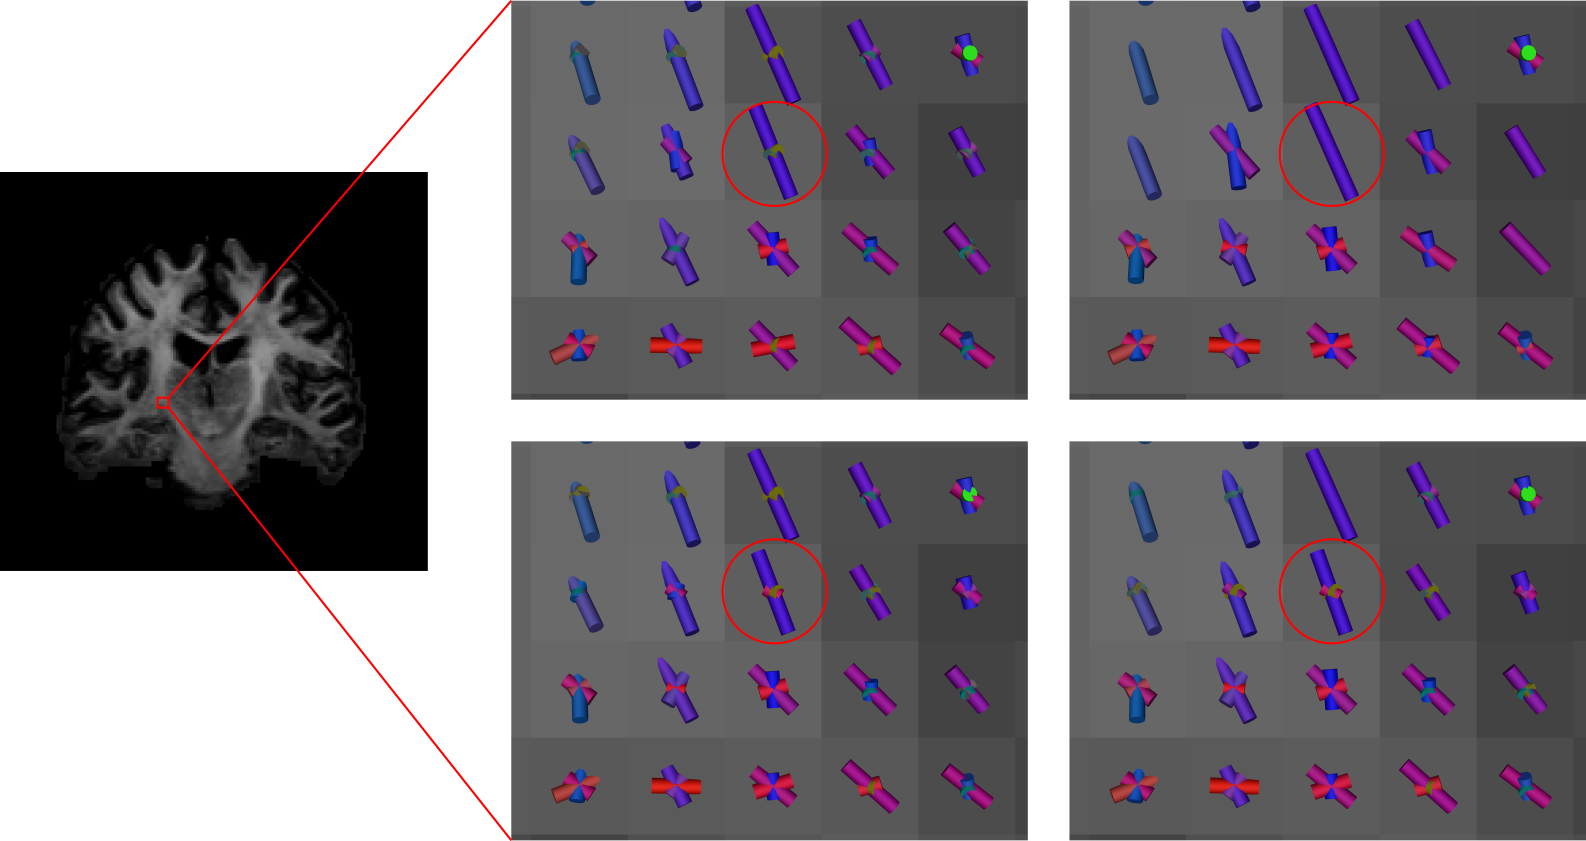
\includegraphics[width=\linewidth]{dir}
	\caption{Reconstructed fiber orientations from the different models. The
          red box in the left image denotes the position within the brain. Both consensus
          models (bottom row) agree quite well in most voxels, although results from model averaging (left) and model selection (right) differ, for example, in the voxel highlighted by the red circle.}
	\label{fig:directions}
\end{figure*}

\begin{figure*}
	\centering
	\begin{minipage}{0.24\linewidth}
\begin{subfigure}[b]{\linewidth}
		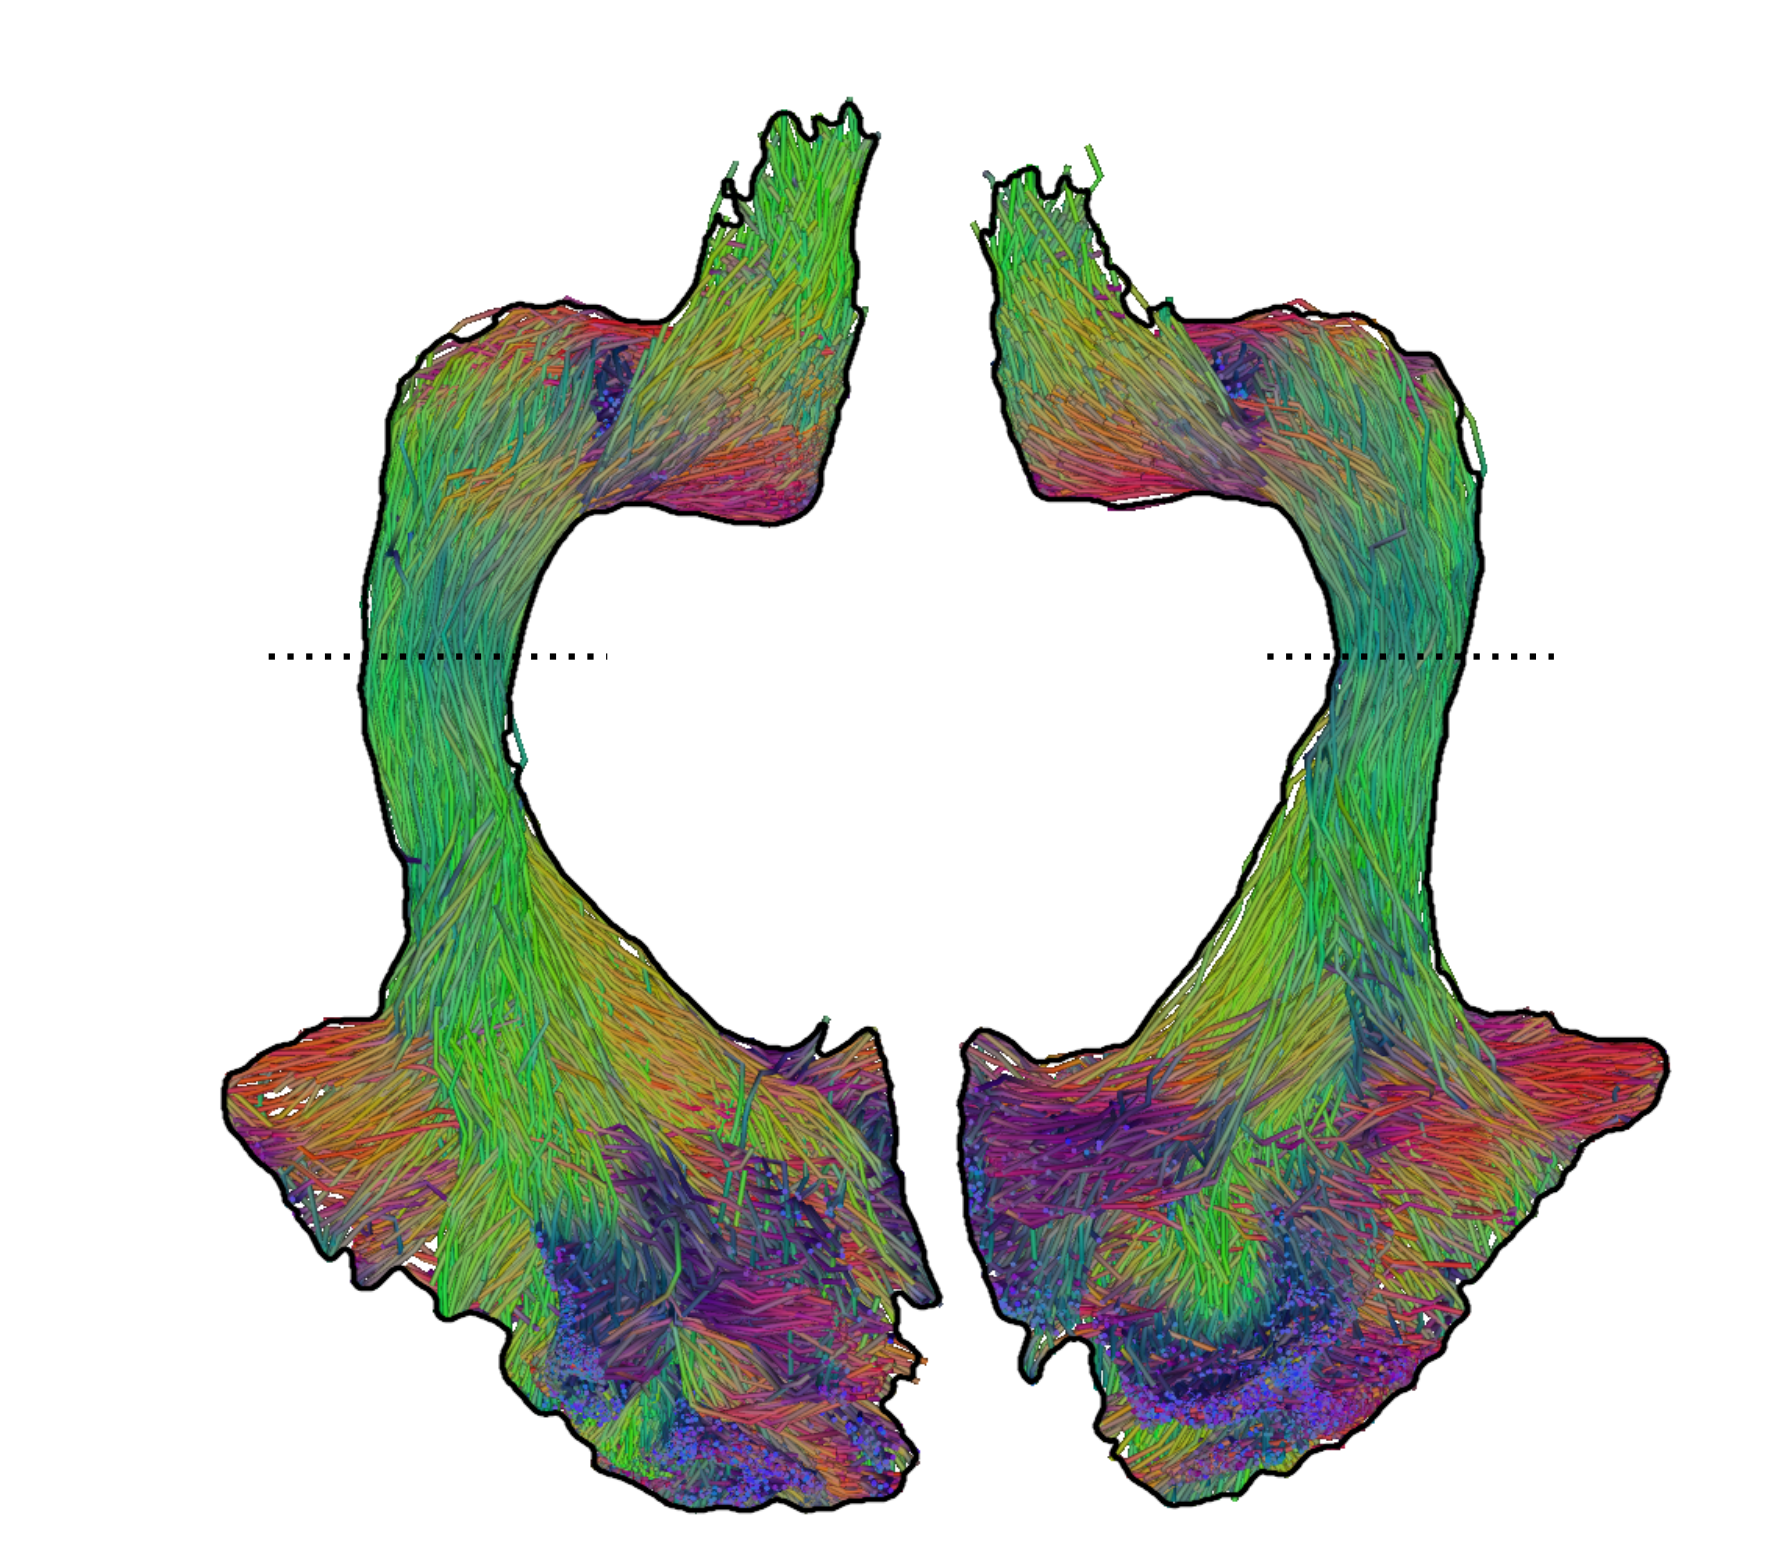
\includegraphics[width=\linewidth]{or-ref-c}
		\caption{Reference {\color{white} avdsdsds} }
	\end{subfigure}
\end{minipage}
\hfil
	\begin{minipage}{0.24\linewidth}
		\begin{subfigure}[b]{\linewidth}
		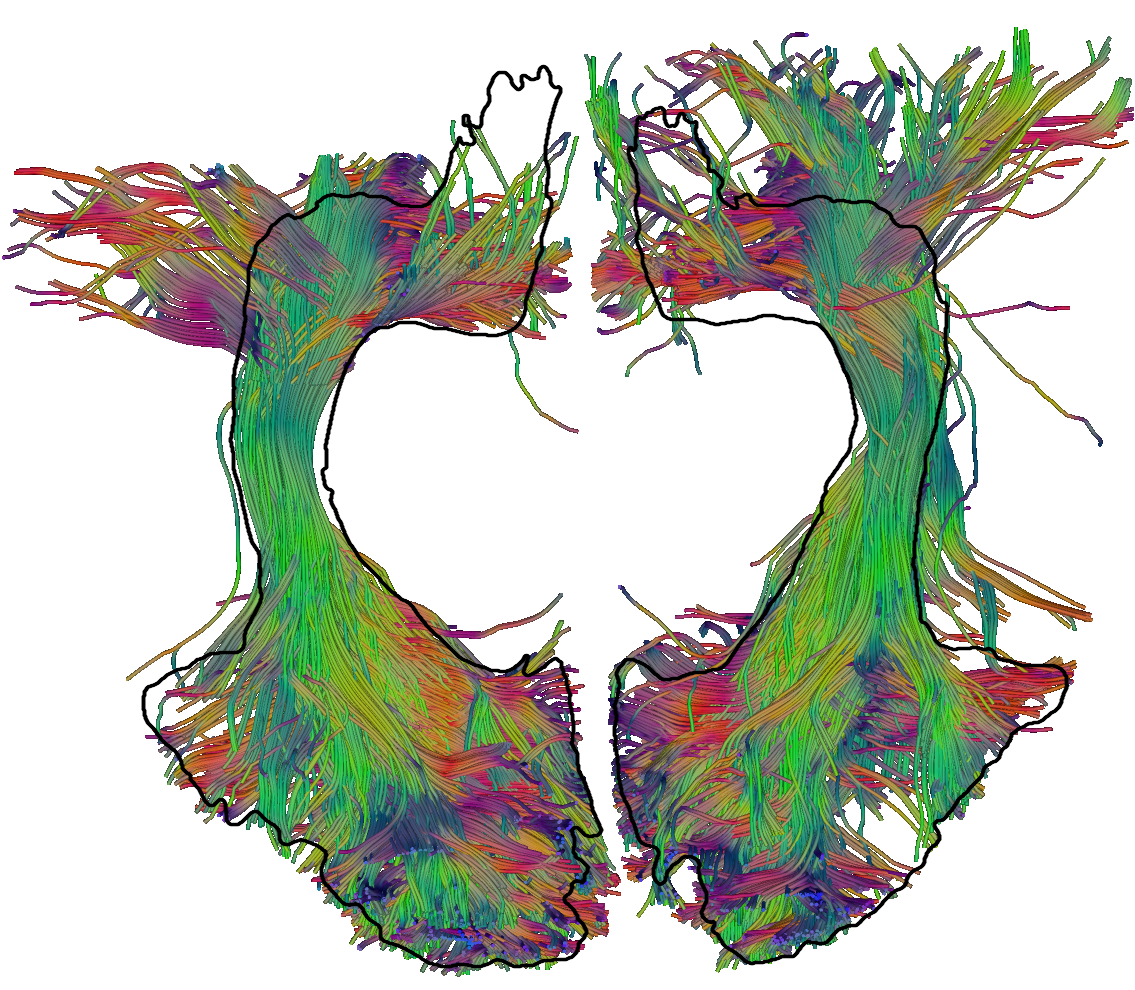
\includegraphics[width=\linewidth]{or-rank-c}
		\caption{Low rank 3 model {\color{white} avdsdsds} }
	\end{subfigure}
	\begin{subfigure}[b]{\linewidth}
		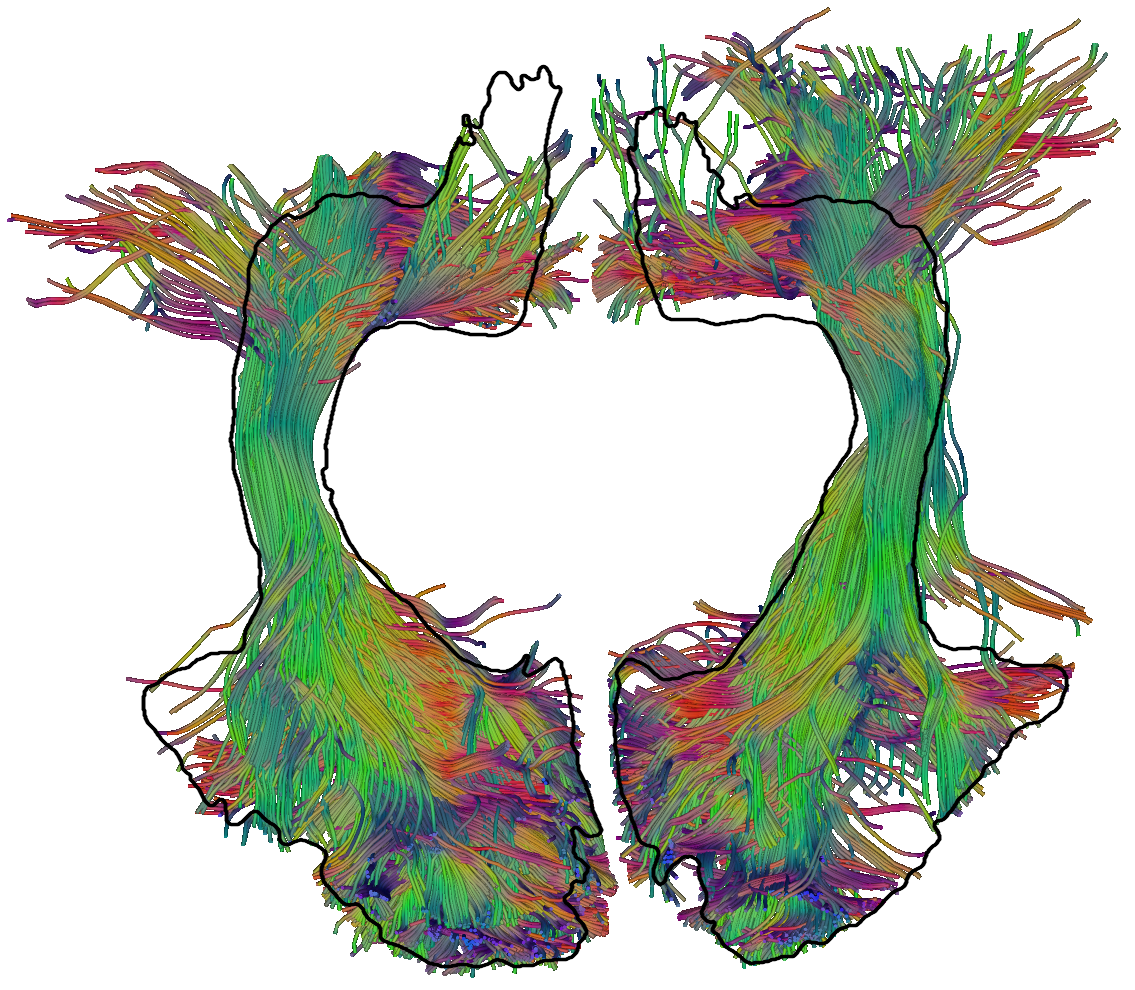
\includegraphics[width=\linewidth]{or-rank-bootstrap-c}
		\caption{Consensus low rank 3 model}
\end{subfigure} 
	\end{minipage} \hfil
	\begin{minipage}{0.24\linewidth}
	\begin{subfigure}[b]{\linewidth}
		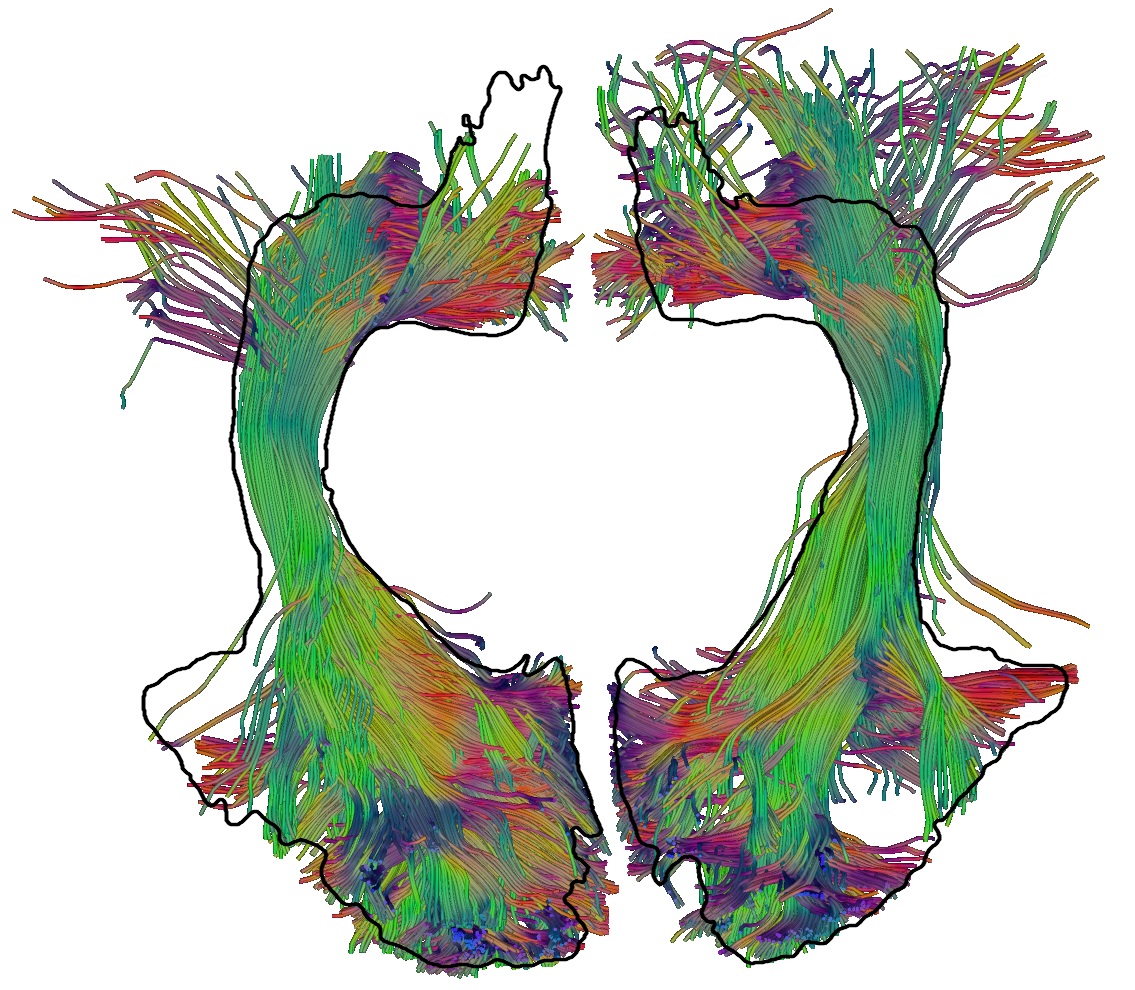
\includegraphics[width=\linewidth]{or-avg-c}
		\caption{Average model {\color{white} aasfd vdsdsds}}
	\end{subfigure}
	\begin{subfigure}[b]{\linewidth}
		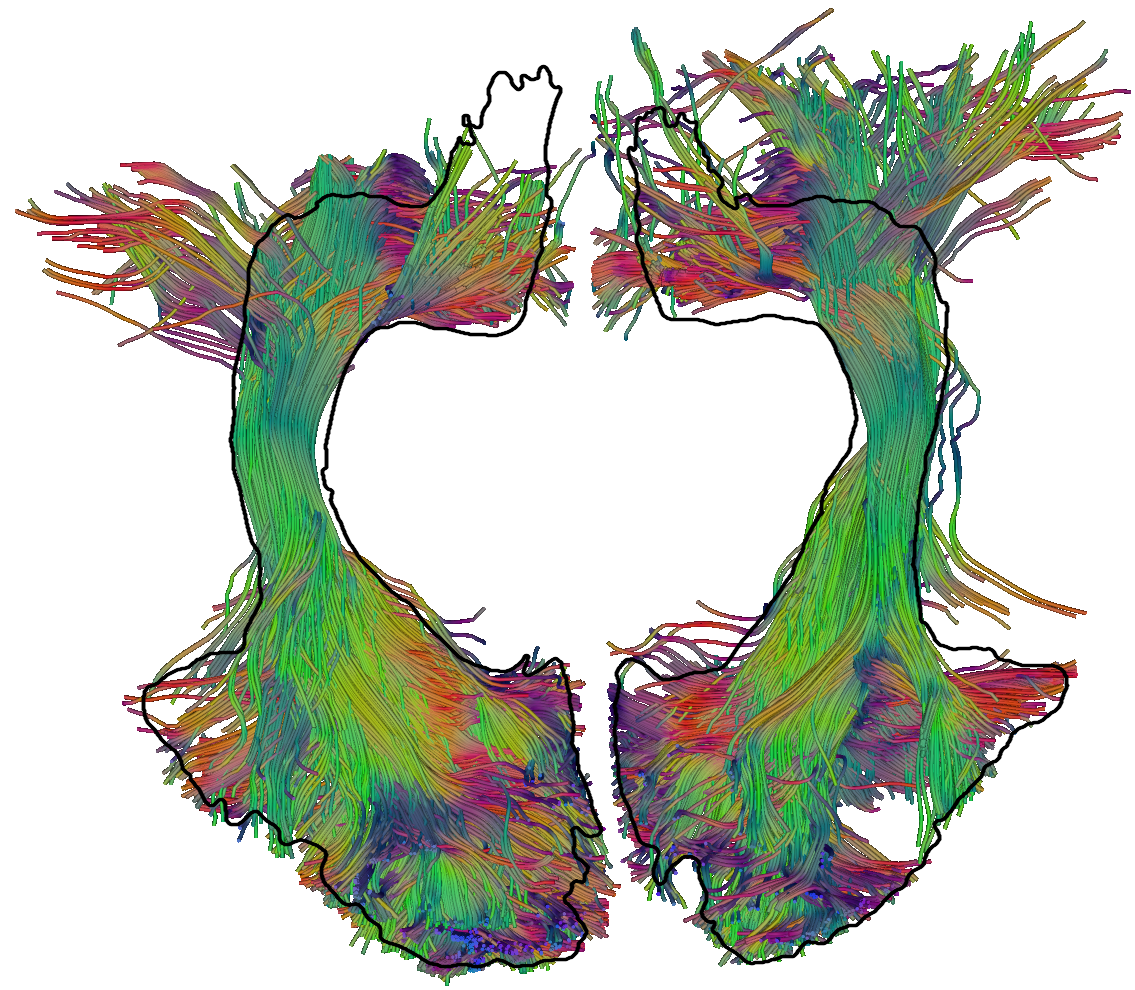
\includegraphics[width=\linewidth]{or-avg-bootstrap-c}
		\caption{Consensus Average model}
\end{subfigure} 
	\end{minipage} \hfil 
	\begin{minipage}{0.24\linewidth} 
	\begin{subfigure}[b]{\linewidth}
		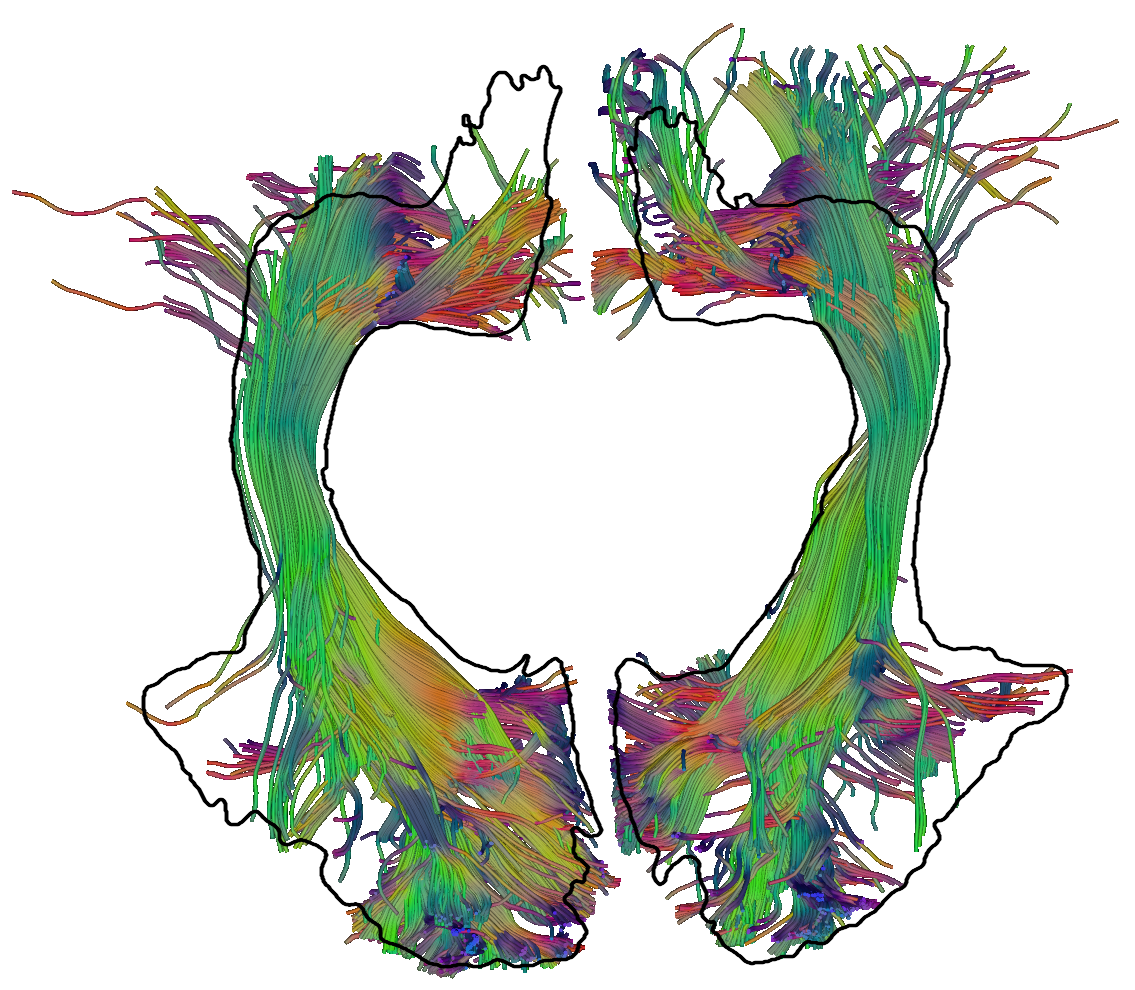
\includegraphics[width=\linewidth]{or-sel-c}
		\caption{Selection model {\color{white} avdsdsds asdf asdf}}
	\end{subfigure}
	\begin{subfigure}[b]{\linewidth}
		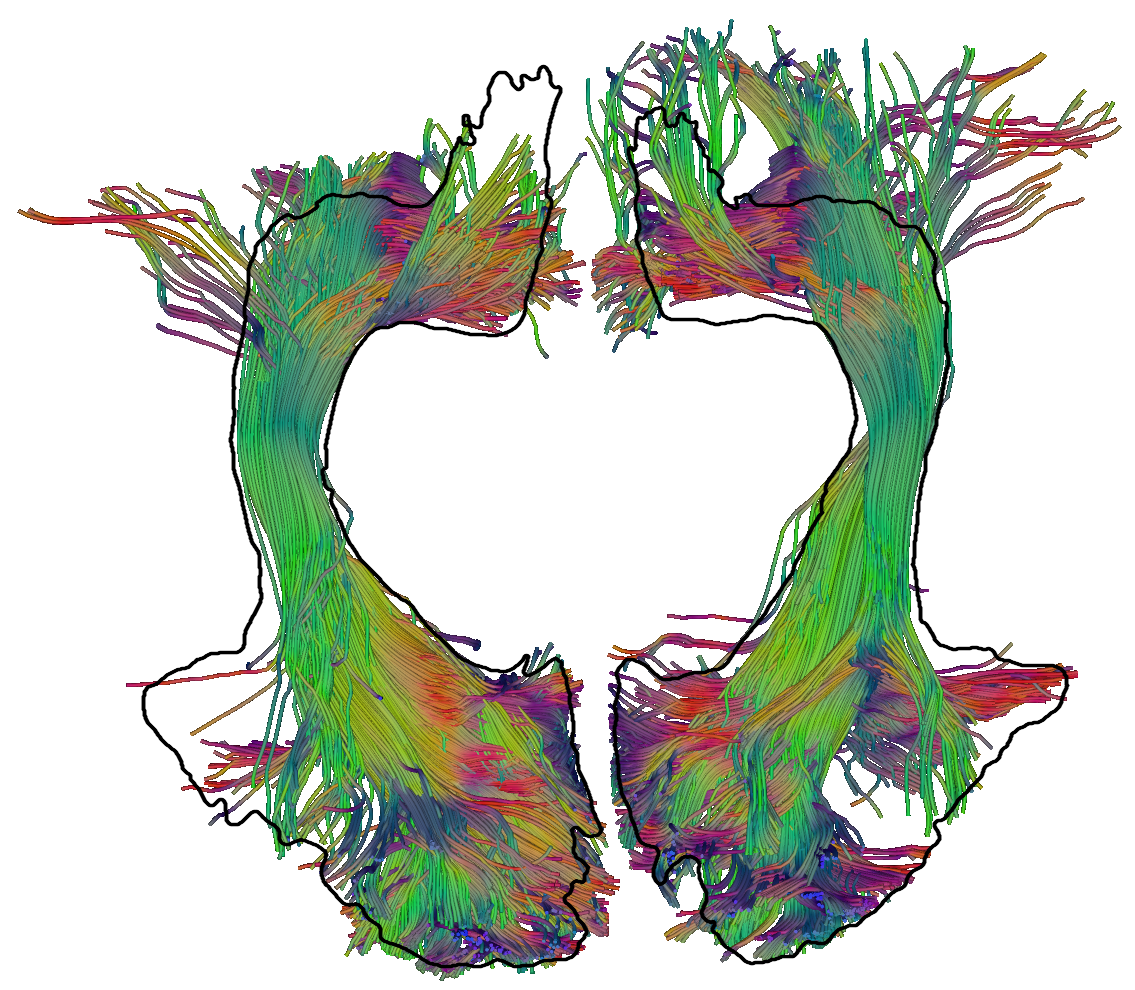
\includegraphics[width=\linewidth]{or-sel-bootstrap-c}
		\caption{Consensus Selection Model}
\end{subfigure} 
	\end{minipage}
	\caption{Reconstruction of the optic radiation (OR). Again, we overlaid the contour of the reference on each reconstruction with a black
          curve. The bootstrap consensus increases the overlap with the reference both for model averaging~(d) and selection~(f). For the rank-3 model~(b), it mostly reduces the false positives, even though that effect is less visible due to the streamline filtering during post-processing.}
	\label{fig:OR}
\end{figure*}

Inspecting the multi vector fields in Fig.~\ref{fig:directions} provides further insight. The most obvious difference between the average and
selection models is that, in many voxels, model averaging (top left) leads to a larger number of fibers compared to model selection (top right). This explains the more complete reconstruction that was observed in Fig.~\ref{fig:CST}. 
On the other hand, applying the bootstrap consensus makes the results from averaging (bottom right) and selection (bottom left) rather similar. The red circle highlights a voxel in which results from model averaging and selection differ, but agree after forming a bootstrap consensus. This illustrates that the bootstrap consensus reduces not just data uncertainty, but also model uncertainty when it is combined with model selection.

Fig.~\ref{fig:OR} provides qualitative results on another bundle, the optic radiation. Model selection~(f) leads to an incomplete reconstruction of the spread in the posterior part, which is again more fully sampled with model averaging. The bootstrap consensus further improves both models.

\subsection{Quantitative Comparison}
\label{sec:quantitative-results}

For a quantitative evaluation, we reconstructed the corpus callosum (CC), the
cingulum (CG), the corticospinal tract (CST), the inferior fronto-occipital (IFO)
and the inferior longitudinal fasciculus (ILF), the optic radiation (OR), and
the superior longitudinal fasciculus (SLF). To keep the analysis more manageable, we combined the left and right tracts, and merged the subtracts that were defined for CC and SLF in the reference \cite{WASSERTHAL2018239}.

\begin{figure}
	\centering
	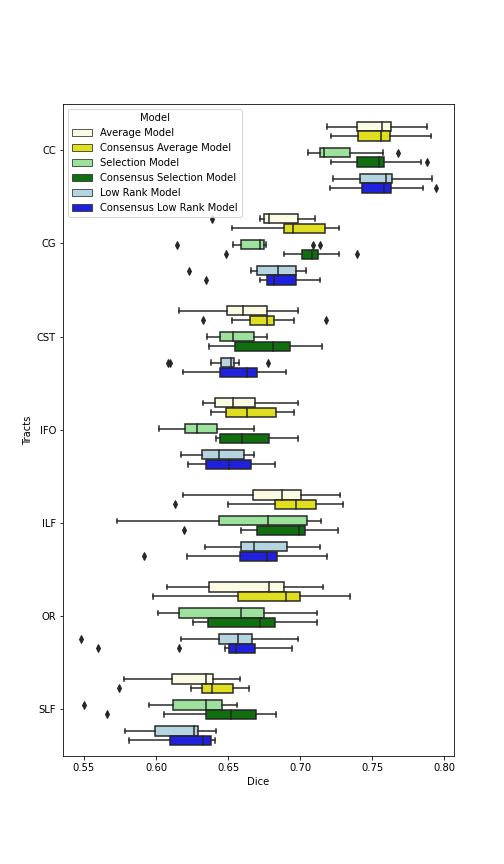
\includegraphics[width=\linewidth]{comparison-dice}
	\caption{Boxplots of the Dice scores of all subjects for all models. In almost all cases, model averaging yields a higher median Dice than model selection, and the bootstrap consensus improves upon the results of the corresponding base model.}
	\label{fig:Dice}
\end{figure}

\begin{table*}
\centering
\begin{tabular}{p{4cm}p{1.5cm}p{1cm}p{1cm}p{1cm}p{1cm}}
	{}  & \rot{Consensus   Average  Model} & \rot{Selection Model} &
	\rot{Consensus Selection Model} & \rot{Rank-3 Model} & \rot{Consensus
	Rank-3 Model} \\ \hline  
Average Model &   {\cellcolor{lightgreen} 0.001} & {\cellcolor{lightred} 0.001}
& {\cellcolor{lightgreen} 0.002} & {\cellcolor{lightred} 0.001} & 0.063 \\
Consensus Average Model &   & {\cellcolor{lightred} 0.001} & 0.900 &
{\cellcolor{lightred} 0.001} & {\cellcolor{lightred} 0.001} \\
Selection Model &    & & {\cellcolor{lightgreen} 0.001} & 0.900 & 0.494 \\
Consensus Selection Model &  &  &  & {\cellcolor{lightred} 0.001} &
{\cellcolor{lightred} 0.001} \\
Rank-3 Model &   &
 &   & & 0.494 \\
\end{tabular}
\caption{Comparison of all models by a Nemenyi post-hoc test. All $p$ values
below $0.05$ are marked in green if the top model is significantly better, else
in red. Our model averaging strategy is significantly better than
model selection and the rank $3$ model. The bootstrap consensus further improves model selection and averaging.}
	\label{tab:sig}
\end{table*}

We
evaluated the reconstruction quality by the Dice score which is defined as
\[ 
	\text{DICE} = \frac{2 |RD \cap TR |}{|TR| + |RD|} ,
\]
where $RD$ denotes a binary mask that is derived from the reference data, and $TR$ a mask from the tracking results
\cite{SCHILLING2019194}. A high Dice score is desired, as it denotes a high
overlap and a low overreach. In Fig.~\ref{fig:Dice}, results from the average,
selection and low-rank model with and without use of the bootstrap consensus are
visualized as box plots to show the tract wise distribution (over subjects) of the Dice scores. In most cases, we observe that model averaging yields a more accurate reconstruction compared to model selection, and that the bootstrap consensus increases Dice compared to the corresponding strategy without bootstrapping.

To further quantify these findings, we compared all six models with a
Friedman test, to investigate whether differences between models are statistically significant \cite{doi:10.1080/01621459.1937.10503522}. Since that was the case ($p\ll 0.001$), we
applied a Nemenyi post-hoc test to identify which models differ significantly
\cite{Nemenyi}.

According to the results of that post-hoc test, which are shown in Table~\ref{tab:sig}, when comparing strategies without the bootstrap consensus,
model averaging is significantly better than either model selection or the rank-3 model, while neither of the latter two are preferable to the other overall. From this, we conclude that model averaging as it was first described in our previous work \cite{Gruen:2021} provides a significant advantage.

Concerning the bootstrap consensus that is introduced in our current work, we observe in Fig.~\ref{fig:Dice} that, in 6 out of 7 tracts, the consensus average model achieves a higher median Dice score than model averaging by itself, that the consensus selection model always beats model selection alone, and that the consensus rank-3 model has a higher median Dice in 4 out of 7
tracts. According to Table~\ref{tab:sig}, these improvements are significant for model averaging and selection, but not for the rank-3 model. We believe this is due to the fact that the main advantage there is to reduce false positive streamlines, most of which are however successfully filtered out before computing the Dice.

Comparing the consensus models with each other, Fig.~\ref{fig:Dice} suggests that the consensus average and selection models are quite similar, and both are
preferable compared to the consensus rank-3 model. This is confirmed by the significance tests. In terms of practical utility, it is relevant to put these results in context with the computational effort of the different approaches.

%Overall we have shown that the consensus model improves our previously proposed
%models significantly. However, the improvement by average Dice score is only for
%the selection model large. 
\subsection{Computational Effort}
\label{sec:computational-effort}
All experiments were computed on an Intel i9 with 3.3~GHz and 64~GB RAM. The
following durations are denoted in (h:)min:s.

The computation of a single bootstrap data sample took 1:10 on a single core,
multi-threaded fourth-order fODF tensor estimation took 4:33, the computation of the multi-vector fields took 0:40 with the rank-3 model, 1:10 with model selection, 1:30 with model averaging. Therefore, the calculation of 100 bootstraps took 8:08:00, using all CPU cores to create the bootstrap data as well as the
models. This also includes the computation of the consensus model, which on its
own took 11:00.

\begin{table}
\centering
\begin{tabular}{p{4cm}p{3cm}}
	{}  & Time per 1000 valid streamlines in seconds\\ \hline  
	Average Model & 27.51\\
	Consensus Average Model & 28.29\\
	Selection Model & 23.70\\
	Consensus Average Model & 24.59 \\
	Rank-3 Model &  43.27\\
	Consensus Rank-3 Model & 35.90\\
\end{tabular}

\caption{Comparison of the average time needed to reconstruct 1000 valid streamlines of
  the right CST in Fig. \ref{fig:CST}. Differences mostly result from the number of successfully filtered false positive streamlines, which do not count towards the valid ones.}
	\label{tab:tracking-times}
\end{table}

Typical times for the tracking itself are reported in Table~\ref{tab:tracking-times}. Times are averages for reconstructing 1000 valid streamlines in the CST. Differences mostly reflect the time spent on tracking false positive streamlines that are discarded by our filters, since those do not contribute towards the valid ones. Here, the fact that the rank-3 baseline generates considerably more false positives becomes even more apparent than in our previous qualitative and quantitative results. Tracking with model selection is fastest, but it is clear from the results above that this comes at the expense of the least complete reconstructions.

%%% Local Variables:
%%% mode: latex
%%% TeX-master: "../main"
%%% End:
